%% LyX 2.3.6.1 created this file.  For more info, see http://www.lyx.org/.
%% Do not edit unless you really know what you are doing.
\documentclass[english]{article}
\usepackage[T1]{fontenc}
\usepackage[latin9]{inputenc}
\setlength{\parskip}{\smallskipamount}
\setlength{\parindent}{0pt}
\usepackage{float}
\usepackage{graphicx}
\usepackage{setspace}
\onehalfspacing
\usepackage{babel}
\begin{document}

\section{Initial Condition}

\subsection{Introduction of Inductivly Coupled Plasma}

Low-pressure high-density plasmas are widely used for semiconductor
processing. High density results in high ion fluxes, which increase
the etch rate. So the throughput of wafer processing can be increased.
Low pressure results in the collision frequency, from which ions reduces
energy loss. So the ion energy to the wafer can be high, benefiting
the desired etch process. Inductively coupled plasma (ICP) meets these
requirements and becomes widely used strting in 1990s. The ``inductively''
in the name comes from the way the electric field is produced. An
electromagnetic field is created by radio frequency (RF) current flowing
in a coil, which can be seen in the figure below. The current flowing
through the coil creates B-field, which in turn creates the E-field
below the dielectric window. The underline E-field delivers the energy
to the electrons, which creates the plasma. The plasma current in
the azimuthal direction also feedbacks to the coil current. Therefore,
the coil and plasma are tightly coupled together.

\begin{figure}[H]
\begin{centering}
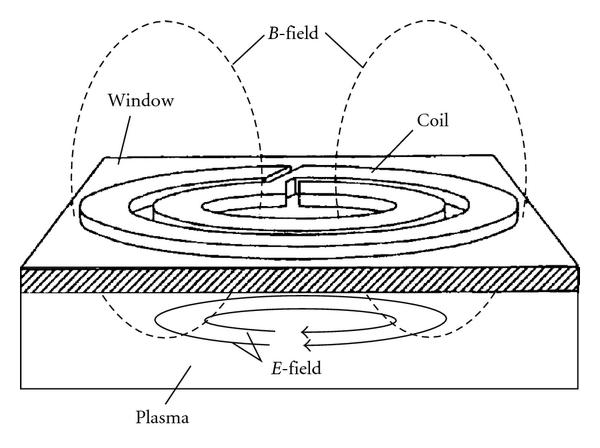
\includegraphics[scale=0.5]{Figures/ICP_Field}
\par\end{centering}
\caption{RF magnetic field (B-field) and RF electric field (E-field) created
inside the ICP by applying RF power to the planar coil through the
dieletric window.}

\end{figure}


\subsection{Model Geometry}

A typical ICP geometry is shown below. The whole domain is defined
by the outmost boundaries. However, the equations in the Reactor Model
are solved in different domains.
\begin{itemize}
\item ICP field equation is solved within the domain except all metals,
plus coils although coils are metal too.
\item Poisson's equation is solved within the domain except all metals.
Coils are not counted.
\item Plasma equation is solved only within the vacuum area, which is the
domian minus all metals and dielectrics.
\end{itemize}
The material properties:
\begin{itemize}
\item Coil current - $I_{coil}$ is determined by the total power coupled
to plasma. It is not easy to determine the initial current value.
Users have to try out in a large range from 0.001 A to 10.0 A.
\end{itemize}
Dieletric constat (relative) (absolute permittivity = $8.85\times10^{-12}m^{-3}kg^{-1}s^{4}A^{2}$
):
\begin{itemize}
\item Vacuum, air - 1.0
\item Quartz - 3.8 - 4.2 depending on what kind of quartz, 4.0 can be used
for most cases
\item Metal - 1.0, metal does not have dieletric constants. It is assigned
1.0 only for computation.
\end{itemize}
Conductivity:
\begin{itemize}
\item Vacuum, air - 0.0
\item Quartz - very small, 1e-6 to 1e-3 S/m. Users can use 0.0. Quartz is
designed to have very small conductivity so that magnetic field can
penetrate through it.
\item Metal - infinity. Metal serves as boundary condition. Users can assign
metal with conductivity of 1.0e6 S/m.
\end{itemize}
\begin{figure}[H]
\begin{centering}
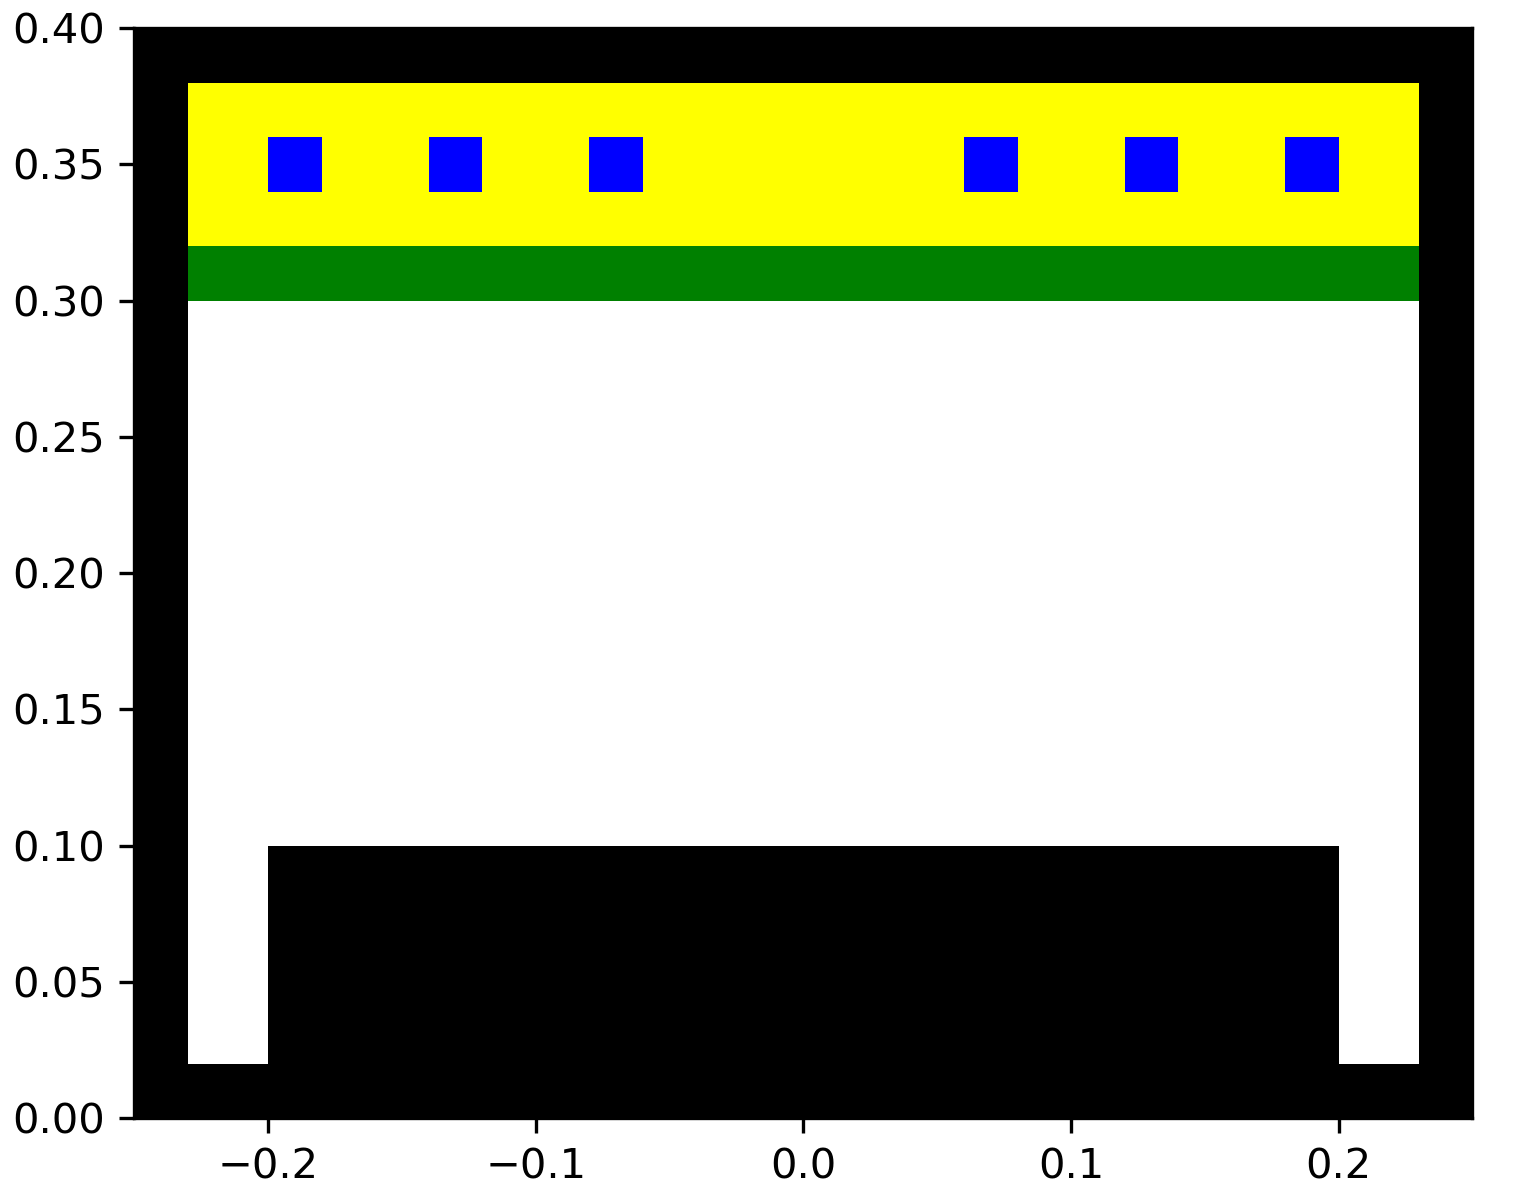
\includegraphics[scale=0.5]{Figures/ICP2D}
\par\end{centering}
\caption{Geometry of an ICP. White - Vacuum; Black - Grounded metal; Blue -
Coil; Yellow - Air; Green - Quartz.}
\end{figure}


\subsection{Initial Condition}

A typical ICP case is given here with all necessary initial conditions,
which can be used as a test for Reactor Model. 

Operation conditions:
\begin{itemize}
\item Pressure - 10 mT
\item Power - 100 W
\item RF frequency - 13.56 MHz
\item Room Temperature - 300 K
\end{itemize}
Plasma conditions:
\begin{itemize}
\item mass - $m_{e}=9.1\times10^{-31}kg,\:m_{Ar}=40\times1.66\times10^{-27}kg$
\item elementary charge - $e=1.6\times10^{-19}\:C$
\item neutral density - $n_{Ar}=P(mT)\times3.3\times10^{19}\:m^{-3}$
\item metastable density - $n_{Ar^{*}}=1\%\times n_{Ar}$
\item electron density - $n_{e}=10^{-4}\times n_{Ar}$
\item ion density - $n_{Ar^{+}}=n_{e}$
\item electron temperature - $T_{e}=1.0\:eV$
\item ion temperature - $T_{Ar^{+}}=0.1\:eV$
\item neutral temperature - $T_{Ar}=T_{Ar^{*}}=0.025\:eV$
\end{itemize}

\end{document}
